% Zhiyunyao/pkuthss: lite LaTeX template for dissertations at Peking University
% 2024/04/26 v1.9.4-lite
% GitHub:   https://github.com/zhiyunyao/pkuthss/tree/lite
% Overleaf: https://www.overleaf.com/read/wmsmytgjkxfy#c888f2

% Copyright (c) 2008-2009 solvethis
% Copyright (c) 2010-2022,2024 Casper Ti. Vector
% Copyright (c) 2021 Kurapica
% Copyright (c) 2022 iofu728
% Copyright (c) 2024 Zhiyunyao

\documentclass[fontset=pkufontauto,zihao=-4,ugly,openany]{pkuthss}
% 字体库      fontset (pkufontauto | pkufontpath)  系统装有宋体等字体请使用 pkufontauto;
%                                  否则使用 pkufontpath 并新建 pkufont 文件夹放置所需字体
% 默认字号     zihao    (-4 | 5)    设定默认字号为小四|五号
% 学位论文模式  ugly   (默认关闭)   打开后论文严格按照学校格式要求编译
% 盲审模式     blind   (默认关闭)   打开后论文按照盲审格式编译
% 英文模式    english  (默认关闭)   打开后论文按照英文格式编译
% 章节新页模式 openany (默认关闭)   每章都从右页(奇数页)开始;打开后每章从任意页开始(禁止章末空白页)
\usepackage{iftex}
\usepackage{xurl}
\def\UrlBreaks{%
    \do\/%
    \do\a\do\b\do\c\do\d\do\e\do\f\do\g\do\h\do\i\do\j\do\k\do\l%
    \do\m\do\n\do\o\do\p\do\q\do\r\do\s\do\t\do\u\do\v\do\w\do\x\do\y\do\z%
    \do\A\do\B\do\C\do\D\do\E\do\F\do\G\do\H\do\I\do\J\do\K\do\L%
    \do\M\do\N\do\O\do\P\do\Q\do\R\do\S\do\T\do\U\do\V\do\W\do\X\do\Y\do\Z%
    \do0\do1\do2\do3\do4\do5\do6\do7\do8\do9\do=\do/\do.\do:%
    \do\*\do\-\do\~\do\'\do\"\do\-}
\urlstyle{same}

% 引入multirow处理表格中的合并单元格
\usepackage{multirow}
% diagbox
\usepackage{diagbox}
% float
\usepackage{float}

\usepackage{amsthm}

\newtheoremstyle{mytheoremstyle}% 请替换为你喜欢的样式名
	{0.5em}% 上间距
	{0.5em}% 下间距
	{}% 定理内容的字体样式
	{}% 缩进量
	{\bfseries}% 定理标题的字体样式
	{:}% 标题后的标点符号
	{0.5em}% 标题与内容之间的距离
	{}% 定理头部的额外规范

{
	\theoremstyle{mytheoremstyle}
	\newtheorem{definition}{定义}[chapter]
	\newtheorem{proposition}{性质}[chapter]
}

\usepackage{algorithm}
\usepackage{algorithmicx}
\usepackage{algpseudocode}

\floatname{algorithm}{算法}
\renewcommand{\algorithmicrequire}{\textbf{输入:}}
\renewcommand{\algorithmicensure}{\textbf{输出:}}
% 参考文献遵循GB/T 7714-2015标准,使用biblatex-gb7714-2015 宏包
% 此处使用顺序编码制,如使用著者-出版年制则更改为b7714-2015ay
\usepackage[backend=biber,style=gb7714-2015,gbnamefmt=lowercase]{biblatex}
\renewcommand*{\bibfont}{\zihao{5}\linespread{1.27}\selectfont}
% 设定参考文献列表的段间距
\setlength{\bibitemsep}{3bp}
% 载入参考文献数据库(注意不要省略“.bib”)
\addbibresource{thesis.bib}

% 示例文档用包和设定,该段均可移除
%\usepackage{enumitem,fancyvrb} % 列表相关
%\usepackage{booktabs,multirow,longtable,makecell} % 表格相关
%\usepackage{hologo} % Tex徽标
%\usepackage{pdfpages}
%\RecustomVerbatimEnvironment{Verbatim}{Verbatim}{frame=single,tabsize=4,fontsize=\footnotesize}
%\renewcommand{\v}[1]{\boldsymbol{#1}}
%\newcommand\pkg[1]{\textsf{#1}}
%\def\liteversion{v1.9.4-lite}
%\def\pkuthss{pkuthss \liteversion}

%% 设定文档基本信息(按照在论文中出现顺序)
% cthesisname: 论文类别,显示在偶数页页眉和pdf文档subject属性,如:
%              北京大学博士学位论文/北京大学硕士学位论文
\cthesisname{北京大学硕士学位论文}
% thesiscover: 封面显示的论文类别
\thesiscover{硕士研究生学位论文}
% ctitlelines: 封面论文标题的下划线行数,设置为0则不在封面显示标题
\ctitlelines{2}
% ctitle: 论文标题,长标题用“\\”强制换行(v1.9.4-lite之前版本“\\”问题已修复)
\ctitle{\pkuthss{} 操作系统内核关键模块的\\形式化验证}
\cauthor{颜森}
\studentid{2201213088}
\school{计算机学院}
\cmajor{计算机软件与理论}
\direction{软件工程与系统软件}
\cmentorlines{1}
\cmentor{赵海燕\;教授}
% degreetype: 1->学术学位,2->专业学位,0->不显示学位类型
\degreetype{1}
% date: 具体时间以教务为准,初稿3月,送审4月,答辩5月,最终6月
\date{二〇二五年五月}
\ckeywords{操作系统验证,形式化验证}

% 英文信息,只在英文摘要页显示
\etitle{\pkuthss{} Formal Verification of Key Modules in Operating System Kernels}
\eauthor{Sen Yan}
\emajor{Computer Software and Theory}
% ementor: 教授 Prof., 副教授 A.P., 讲师 Lec.
\ementor{Prof. Haiyan Zhao}
\ekeywords{Operating System Verification, Formal Verification}

%% 盲审信息,只在盲审模式显示,无盲审需求的用户可忽略
% discipline: 一级学科(cmajor是二级学科)
\discipline{计算机软件与理论}
% blindid: 盲审论文编号
\blindid{9876543210}

%% 设定论文元素名称
\ctexset{
    % appendixname   = {附录},
    % bibname        = {参考文献},
    % contentsname   = {目录},
    listtablename  = {表格索引},
    listfigurename = {插图索引},
    % figurename     = {图},
    % tablename      = {表}
}

%% 设定链接显示效果
\hypersetup{
    hidelinks,                   % 移除链接的字体颜色和边框
    linktoc            = all,    % 目录设置为链接的级别 (none | section | page | all)
    breaklinks         = true,   % 是否允许链接换行
    pdfdisplaydoctitle = true,   % 是否在文件标题属性展示标题而不是文件名
    bookmarksdepth     = 3,      % pdf 书签最大深度
    bookmarksopen      = true,   % pdf 书签是否自动展开
    bookmarksopenlevel = 1       % pdf 书签自动展开级别
}%

\begin{document}
    %% 以下为正文之前的部分,默认不进行章节编号
    \frontmatter
    % 此后到下一 \pagestyle 命令之前不排版页眉或页脚
    \pagestyle{empty}
    % 自动生成封面
    \maketitle
    % 封面要求单面打印,故须新开右页
	\cleardoublepage
    % 此处不用 \specialchap,因为学校要求目录不包括其自己及其之前的内容。
\chapter*{版权声明}
% 综合学校的书面要求及 Word 模版来看,版权声明页不用加页眉、页脚。
\thispagestyle{empty}

任何收存和保管本论文各种版本的单位和个人,
未经本论文作者同意,不得将本论文转借他人,
亦不得随意复制、抄录、拍照或以任何方式传播。
否则,引起有碍作者著作权之问题,将可能承担法律责任。

% 若须排版二维码,请将二维码图片重命名为“barcode”,
% 转为合适的图片格式,放在 fig 目录下,然后去掉下面 2 行的注释。
% \vfill\noindent
% \includegraphics[height = 5em]{fig/barcode}

    % \includepdf{./filename.pdf}

    %% 此后到下一 \pagestyle 命令之前正常排版页眉和页脚
    \cleardoublepage
    \pagestyle{plain}
    % 重置页码计数器,用大写罗马数字排版此部分页码
    \setcounter{page}{0}
    \pagenumbering{Roman}
    % 中英文摘要
    % Copyright (c) 2014,2016,2021 Casper Ti. Vector
% Public domain.
\begin{cabstract}
\indent 形式化验证是确保操作系统内核正确性、安全性和可靠性的重要手段。本研究基于霍尔逻辑(Hoare Logic)及其扩展——分离逻辑(Separation Logic),结合Coq证明助手,开展了一项操作系统内核形式化验证的工程实践,重点验证了内存管理、进程隔离和并发同步等关键模块的正确性。通过分离逻辑的资源分离特性,我们清晰地描述并验证了内核模块的资源使用情况,避免了资源冲突和竞争条件。针对并发环境的复杂性,我们采用并发分离逻辑(Concurrent Separation Logic),确保了多线程环境下资源共享与同步机制的正确性。借助Coq的交互式证明机制,我们从高层规约逐步精化并验证了内核实现,确保其与规约的一致性。\\
\indent 本文首先分析了操作系统形式化验证的研究现状,总结了定理证明、模型检测和符号执行等方法在操作系统验证中的应用场景及其局限性。随后,详细介绍了霍尔逻辑和分离逻辑的基本原理及其在形式化验证中的优势,特别是分离逻辑在描述动态内存分配和并发资源共享方面的表达能力。在此基础上,我们基于工程实践,利用分离逻辑对操作系统内核的关键功能模块进行了形式化规约与验证,重点验证了内存管理和并发同步机制的正确性。\\
\indent 在验证过程中,我们充分利用分离逻辑的资源分离特性,清晰地描述和验证了内核中不同模块的资源使用情况,避免了资源竞争和冲突。针对并发环境下的复杂性,我们引入了并发分离逻辑(Concurrent Separation Logic),验证了多线程环境下的资源共享与同步机制的正确性。通过Coq证明助手的交互式证明机制,我们逐步完成了从高层规约到低层实现的精化验证,确保了内核代码与规约的一致性。\\
\indent 本研究的贡献主要体现在以下几个方面:
\begin{itemize}
    \item 基于分离逻辑和Coq证明助手,实现了操作系统内核关键模块的形式化验证,为高可信操作系统的工程实践提供了参考。
    \item 验证了分离逻辑在操作系统形式化验证中的实用性,特别是在内存管理和并发同步方面的优势。
    \item 通过工程实践,展示了形式化验证在操作系统验证和开发中的实际应用价值,为后续研究提供了经验。
\end{itemize}
\indent 本研究为操作系统形式化验证的工程实践提供了具体案例,对推动高可信操作系统的开发具有重要意义。
\end{cabstract}
\begin{eabstract}
\indent Formal verification of operating systems (OS) is a critical approach to ensuring the correctness, security, and reliability of OS kernels. Traditional testing methods often fall short of comprehensively addressing potential errors in complex systems, while formal verification employs mathematical techniques to rigorously prove that a system adheres to its specifications. This study focuses on an engineering practice of formal verification for OS kernels, utilizing Hoare Logic and its extension, Separation Logic, along with the Coq proof assistant. The practice specifically targets the verification of key kernel modules, including memory management, process isolation, and concurrent synchronization mechanisms.\\
\indent The paper begins by reviewing the state of the art in OS formal verification, summarizing the applications and limitations of theorem proving, model checking, and symbolic execution in this domain. It then introduces the foundational principles of Hoare Logic and Separation Logic, highlighting the latter's strengths in describing dynamic memory allocation and shared resource management in concurrent environments. Building on these principles, the study conducts formal specification and verification of critical OS kernel modules based on practical engineering requirements.\\
\indent In this engineering practice, Separation Logic's resource separation properties are leveraged to clearly describe and verify resource usage across different kernel modules, preventing resource conflicts and race conditions. For handling concurrency complexities, Concurrent Separation Logic is employed to verify the correctness of resource sharing and synchronization mechanisms in multi-threaded environments. Using Coq's interactive proof mechanisms, the practice incrementally refines and verifies the kernel implementation against its high-level specifications, ensuring consistency between the code and its formal model.\\
\indent The contributions of this study are mainly reflected in the following aspects:
\begin{itemize}
    \item formal verification of critical OS modules using Separation Logic and Coq, providing a practical reference for high-assurance OS development.
    \item a demonstration of Separation Logic's effectiveness in memory management and concurrency.
    \item a real-world case study highlighting the value of formal verification in OS engineering.
\end{itemize}
\indent This work contributes to advancing reliable OS development and lays the groundwork for future research on scalable and automated verification techniques.
\end{eabstract}

% vim:ts=4:sw=4
    % 自动生成目录
    \tableofcontents
    % 如有需要自动生成表格索引、插图索引
    \listoftables

    \listoffigures
    % 如有需要生成主要符号对照表
    %\begin{denotation}

    \item[$x,y,m,n,t$] 标量,通常为变量
    \item[$K,L,D,M,N,T$] 标量,通常为超参数
    \item[$x\in \mathbb{R}^{D}$] D维列向量
    \item[$(x_1,\cdots,x_D)$] D维行向量
    \item[$(x_1,\cdots,x_D)^T$ or $(x_1;\cdots;x_D)^T$]  D维行向量
    \item[$\v A\in \mathbb{R}^{K\times D}$]  大小为$K\times D$的矩阵
    \item[$x\in \mathbb{R}^{KD}$]  ($KD$)维的向量
    \item[$\mathbb{M}_i$ or $\mathbb{M}_i(\v x)$]  第$i$列为$\v 1$(或者$\v x$),其余为$\v 0$的矩阵
    \item[$diag(\v x)$]  对角矩阵,其对角元素为$\v x$
    \item[$\v I_N$ or $I$]  ($N\times N$)的单位阵
    \item[$diag(\v A)$]  列向量,其元素为$\v A$的对角元素
    \item[$\v A \in \mathbb{R}^{D_1\times D_2\times \cdots \times D_K}$]  大小为$D_1\times D_2\times \cdots \times D_K$的张量
    \item[$\{x^{(n)}\}^{N}_{n=1}$]  集合
    \item[$\{(x^{(n)},y^{(n)})\}^{N}_{n=1}$]  数据集
    \item[$\mathcal{N}(\v x;\mu,\sum)$]  变量$x$服从均值为$\mu$,方差为$\sum$的高斯分布

\end{denotation}

\footnotetext[1]{本符号对照表内容选自\citeauthor{qiu2020nndl}老师的《神经网络与深度学习》\cite{qiu2020nndl}一书。}


    %% 以下为正文部分,默认要进行章节编号
    \mainmatter
    \chapter{引言}
\section{研究背景}
这是研究背景
\section{研究内容和意义}
\section{相关研究工作}
\section{文章结构}
    \chapter{相关理论基础与工具}
\section{程序验证方法概述}

软件工程领域确保程序正确性的方法主要分为动态方法和静态方法两类。动态方法需要将源代码编译为可执行文件,通过运行程序并输入测试用例来观察结果。这类方法的典型代表是软件测试,包括人工执行的单元测试和自动化的模糊测试。动态方法的优势在于能够快速定位具体错误,但其局限性也非常明显:首先,测试必须依赖可运行的环境;其次,由于程序执行路径和输入组合的复杂性,测试无法覆盖所有可能性,只能验证已执行路径的正确性,无法证明整个程序不存在缺陷。

静态方法通过直接分析源代码来验证程序属性,无需实际运行程序。常见的静态方法包括静态分析、符号执行、定理证明和模型检测等。其中,常规静态分析技术(例如Coverity工具)虽然能快速扫描大规模代码,但会产生较高比例的误报结果,需要人工二次验证。符号执行技术通过符号化变量模拟程序执行路径,利用约束求解器验证路径可达性,但在处理循环结构和复杂分支时容易引发路径爆炸问题。定理证明方法要求开发者使用高阶逻辑形式化描述程序规范,并通过交互式工具(如Coq)逐步完成证明,这种方法虽然数学严谨,但需要投入大量专业人力资源,难以适应快速迭代的开发需求。程序验证作为静态方法的延伸,专注于自动化证明程序的基础安全属性(如内存安全、无除零错误等),其效果依赖于约束求解算法的持续优化。

\subsection{操作系统关键模块形式化验证的动机与依据}

操作系统内核中进程调度、内存管理和中断处理等关键模块的可靠性直接决定了整个系统的安全性。本文选择形式化验证方法主要基于以下三方面原因:
\begin{itemize}
    \item 传统测试方法存在本质缺陷。以Linux内核为例,历史漏洞中有三分之一以上涉及内存管理模块,而这些漏洞大多无法通过常规测试发现。内核模块需要处理硬件中断、多线程调度等复杂并发场景,其执行路径数量随线程数增长呈指数级上升,动态测试难以覆盖所有可能性。此外,内核与硬件设备的深度耦合导致测试结果严重依赖特定环境,难以保证验证结论的普适性。
    \item 形式化验证具有数学完备性优势。该方法通过建立形式化模型对程序行为进行严格推演,能够覆盖所有可能的执行路径。例如,seL4微内核项目使用Isabelle/HOL工具验证了内核代码不存在缓冲区溢出等安全漏洞,微软使用TLA+语言验证了Hyper-V虚拟化平台的并发调度算法。对于硬件交互场景,形式化方法可通过抽象寄存器传输模型验证中断处理时序等关键属性,这是传统方法无法实现的。
    \item 操作系统关键模块的特性适合形式化验证。现代微内核架构(如Zircon)将核心功能拆分为独立模块,降低了形式化建模的复杂度。同时,内核模块的代码规模通常控制在数万行以内,且更新频率较低,能够平衡验证成本与长期收益。工业界实践表明,对安全关键模块实施形式化验证的整体成本,仅为后期修复漏洞成本的15\%-20\%,具备显著的经济可行性。
\end{itemize}

\section{形式化验证方法概述}
\label{sec:formal-methods}
形式化验证是一种基于数学逻辑的严格验证技术,通过形式化建模、规约描述和自动化推理,证明系统满足其设计需求。其核心目标是消除自然语言描述的歧义性,并确保系统的正确性、安全性和可靠性。根据验证方法和工具的不同,形式化验证主要分为以下四类:
\begin{enumerate}
    \item \textbf{定理证明}:基于数理逻辑(如霍尔逻辑、分离逻辑)构建形式化规约,通过交互式推导验证系统性质,擅长处理并发、资源管理等复杂逻辑,但依赖人工指导,代表工具有Coq、Isabelle;
    \item \textbf{模型检测}:遍历有限状态空间验证时态逻辑规约,全自动化但受限于状态爆炸问题,适用于硬件协议验证;
    \item \textbf{符号执行}:将程序输入抽象为符号变量进行路径探索,可检测边界条件错误,但对并发同步验证能力有限;
    \item \textbf{静态分析}:通过抽象解释等技术检测代码缺陷,高效但存在误报。在操作系统内核验证中,定理证明因其对动态内存管理、进程隔离等非平凡性质的严格证明能力成为首选方法。
\end{enumerate}

本研究基于分离逻辑与Coq/VST-IDE工具链,通过霍尔逻辑的扩展实现对鸿蒙LiteOS-m内核的形式化验证。

\subsection{一阶谓词逻辑}
一阶谓词逻辑是由逻辑命题扩展而来,并增加了全称量词和存在量词。一阶谓词逻辑存在可靠且完备的演绎系统,显著增强了逻辑表达能力。其核心扩展特性如下:
\begin{enumerate}
    \item \textbf{语法扩展}:在命题逻辑基础上引入:
    \begin{itemize}
        \item \textbf{量词}:引入了全称量词($\forall$)与存在量词($\exists$)
        \item \textbf{谓词}:方便用于描述对象间关系(如$Alloc(ptr)$表示指针$ptr$已分配内存)
        \item \textbf{个体域}:同时也可以表示变量取值范围(如进程集合、内存地址空间)
    \end{itemize}
    
    \item \textbf{可靠性与完备性}:
    \begin{itemize}
        \item \textbf{可靠性}:证明公式均为逻辑有效式($\vdash \phi \implies \models \phi$)
        \item \textbf{完备性}:通过哥德尔定理可以保证所有逻辑有效式均可被证明($\models \phi \implies \vdash \phi$)
    \end{itemize}
    
    \item \textbf{在形式化验证中的应用}:
    \begin{itemize}
        \item 可以用于描述系统全局不变式:
        \begin{equation*}
          \forall p{\in}Process,\ \forall m{\in}Memory,\ 
          \mathit{Owns}(p, m) \to \lnot \exists q{\neq}p,\ \mathit{Owns}(q, m)
        \end{equation*}
        \item 可以作为霍尔逻辑与分离逻辑的底层断言语言
    \end{itemize}

    \item \textbf{局限性}:
    \begin{itemize}
        \item 难以直接表达动态资源管理(需扩展为分离逻辑)
        \item 无法描述高阶性质(如程序终止性)
    \end{itemize}
\end{enumerate}

在鸿蒙LiteOS-m验证中,一阶逻辑用于定义进程隔离与内存权限的抽象规约,其可靠性与完备性为后续霍尔逻辑和分离逻辑的验证框架提供了理论保证。

\subsection{霍尔逻辑与分离逻辑}
\label{subsec:hoare-separation}

霍尔逻辑与分离逻辑构成操作系统内核形式化验证的理论核心,二者通过逐层扩展解决了程序正确性验证中的关键挑战。

\subsubsection{霍尔逻辑的形式化框架}
霍尔逻辑通过\textbf{霍尔三元组} $\{P\}\;C\;\{Q\}$ 描述程序片段 $C$ 的前后状态约束,其中:
\begin{itemize}
    \item 其中,$P$和$Q$是一阶逻辑公式,分别表示前置条件(Pre-Condition)和后置条件(Post-Condition)。 $C$表示一段程序源代码。 霍尔三元组的含义是,假定前置条件是有效的,那么在执行完程序后,后置条件将会是有效的。
    \item 推导规则(如顺序组合、条件分支、循环不变式)构成程序语义的公理化系统。
\end{itemize}
\subsection{霍尔逻辑的推理规则}
在介绍霍尔逻辑的推理规则前,需要先说明推理规则(Inference Rule)的符号表示。推理规则一般表示为以下形式:

$$
\text{Name} \quad \frac{C_1 \quad C_2 \quad \cdots}{R}
$$

其中:
\begin{itemize}
    \item 左侧的 \text{Name} 表示规则名称
    \item 横线上方的 $C_1, C_2, \ldots$ 表示前提条件
    \item 横线下方的 $R$ 表示结论
\end{itemize}

该表示形式意味着:当满足前提条件 $C_1, C_2, \ldots$ 时,通过 \text{Name} 规则可以推导出结论 $R$。

例如:
$$
\text{Apply} \quad \frac{A \quad A \Rightarrow B}{B}
$$

当存在前提条件 $A$ 和 $A \Rightarrow B$ 时,即可通过 Apply 规则推导出 $B$ 成立。

\subsubsection{分离逻辑的扩展机制}
传统霍尔逻辑难以建模动态内存操作(如指针别名、堆内存分配)。分离逻辑通过引入\emph{分离合取}($\sepcon$)与\emph{空间资源模型},扩展了霍尔逻辑的表达能力:
\begin{itemize}
    \item \textbf{分离合取}:断言$P \sepcon Q$表示资源被划分为互不相交的$P$和$Q$两部分,满足:
    \begin{equation}
        \mathcal{H} \models P \sepcon Q \iff \exists \mathcal{H}_1, \mathcal{H}_2,\ \mathcal{H} = \mathcal{H}_1 \uplus \mathcal{H}_2 \land \mathcal{H}_1 \models P \land \mathcal{H}_2 \models Q
    \end{equation}
    
    \item \textbf{堆操作公理}:内存分配规则形式化为:
    \begin{equation}
        \inferrule*[right=Alloc]{
            \mathrm{emp}
        }{
            \hoare{\mathrm{emp}}{\mathtt{alloc}(n)}{\exists p.\, p \mapsto \_ \ast \mathrm{block}(p, n)}
        }
        \end{equation}
    其中$\mathrm{emp}$表示空堆,$p \mapsto \_\,$声明指针$p$的有效性,$\mathrm{block}(p, n)$表示从$p$起始的$n$字节连续内存块;
    
    \item \textbf{局部性原理}:程序验证满足框架规则:
    \begin{equation}
        \inferrule*[right=Frame]{}{\hoare{P}{C}{Q} \implies \hoare{P \sepcon R}{C}{Q \sepcon R}}
    \end{equation}
\end{itemize}

\subsubsection{并发分离逻辑的同步机制}
\label{subsubsec:concurrent-logic}

基于\cite{brookes2007concurrent}的并发分离逻辑框架,多线程环境下的同步机制通过以下三个核心要素实现:

\begin{itemize}
    \item \textbf{资源划分公理}:
    \begin{itemize}
        \item \emph{独占资源}:线程私有资源通过分离合取符$\sepcon$隔离,满足:
            \begin{equation}
                \mathrm{Own}(t, R) \sepcon \mathrm{Own}(t', R') \vdash t \neq t' \rightarrow R \sepcon R'
            \end{equation}
        \item \emph{共享资源}:需通过锁保护的共享资源,满足全局不变式$I$
    \end{itemize}

    \item \textbf{锁机制推理规则}:
    \begin{itemize}
        % Acquire规则
        \item 锁获取规则:
            \begin{equation}
            \inferrule*[right={\normalfont (Acquire)}]{
                \mathrm{Lock}(l, R) \sepcon P
            }{
                \hoare{\mathrm{Lock}(l, R) \sepcon P}{\mathtt{acquire}(l)}{R \sepcon P}
            }
            \label{eq:acquire-rule}
            \end{equation}
        
        % Release规则
        \item 锁释放规则:
            \begin{equation}
            \inferrule*[right={\normalfont (Release)}]{
                R \sepcon P
            }{
                \hoare{R \sepcon P}{\mathtt{release}(l)}{\mathrm{Lock}(l, R) \sepcon P}
            }
            \label{eq:release-rule}
            \end{equation}
    \end{itemize}

    \item \textbf{共享不变式约束}:
        \begin{equation}
            \mathrm{Lock}(l, R) \triangleq l \hookrightarrow \mathrm{locked} \ast R \ast I
            \label{eq:lock-inv}
        \end{equation}
        其中$I$为锁保护的全局不变式,需满足:
        \begin{itemize}
            \item 互斥性:$I \sepcon I \vdash \bot$
            \item 持久性:$I$在锁操作前后保持成立
        \end{itemize}

    \item \textbf{线性所有权传递}:通过移动语义(Move Semantics)确保资源所有权的线程间转移不可复制,例如:
        \begin{equation}
            \mathrm{Chan}(c, m) \vdash \neg \exists m'.\, \mathrm{Chan}(c, m') 
        \end{equation}
\end{itemize}

\subsubsection{在操作系统验证中的适用性}
在鸿蒙LiteOS-m内核验证中,分离逻辑解决了以下关键问题:
\begin{itemize}
    \item \textbf{内存管理}:通过$\mathrm{block}(p, n)$与$\sepcon$验证堆分配器的空间隔离性;
    \item \textbf{进程隔离}:利用资源分离性证明进程间内存与硬件资源的无冲突访问;
    \item \textbf{并发同步}:基于$\mathrm{Lock}(l, R)$断言验证自旋锁与信号量的互斥性与无死锁性。
\end{itemize}

霍尔逻辑与分离逻辑的逐层扩展,为操作系统内核的形式化验证提供了兼具严谨性与实用性的理论工具。
\subsection{操作系统验证中的应用}
\label{subsec:os-verification}

操作系统内核的形式化验证是确保其可靠性、安全性和功能正确性的关键手段。本节基于霍尔逻辑与分离逻辑的理论框架,结合定理证明与自动化工具链,阐述形式化验证在操作系统内核中的典型应用场景。

\subsubsection{内核关键模块的验证目标}
\begin{itemize}
    \item \textbf{内存管理}:验证动态内存分配/释放的安全性(如无野指针、无内存泄漏),满足分离逻辑的堆分离性($\mathrm{block}(p, n) \sepcon \mathrm{valid}(p)$);
    \item \textbf{进程隔离}:保证进程间资源(内存、文件句柄)的独占性,形式化描述为:
        \begin{equation}
            \forall p_1 \neq p_2,\ \mathrm{Res}(p_1) \sepcon \mathrm{Res}(p_2)
        \end{equation}
    \item \textbf{并发同步}:通过并发分离逻辑的$\mathrm{Lock}(lk, R)$不变式实现对锁、信号量等同步原语的原子性与无死锁性的验证。
\end{itemize}

\subsubsection{形式化验证方法论}
\begin{itemize}
    \item \textbf{定理证明}:基于Coq的交互式证明,从高层规约逐步精化至C代码实现(如seL4微内核验证);
    \item \textbf{模型检测}:针对有限状态子系统(如调度算法),使用TLA+或SPIN验证时态逻辑性质(如无饥饿性);
    \item \textbf{符号执行}:结合KLEE等工具验证系统调用的路径可达性与边界条件。
\end{itemize}

\subsubsection{工具链协同验证流程}
现有操作系统内核验证通常遵循以下工程实践:
\begin{enumerate}
    \item \textbf{规约层}:定义内核的安全属性、正确性要求,并使用形式化语言建立数学模型。
    \item \textbf{代码层}:使用受限的语言或严格的编码风格,使代码能够直接与规约保持一致,以便验证。
    \item \textbf{证明层}:使用形式化证明工具确保代码实现符合规约,保证内核的安全性和正确性。
    \item \textbf{硬件适配}:确保操作系统能在实际硬件上安全、高效地运行,并验证硬件相关的安全性质。
\end{enumerate}

\subsubsection{挑战与解决方案}
\begin{itemize}
    \item \textbf{状态空间爆炸}:通过模块化验证(如分离逻辑的局部性原理)分解系统复杂度;
    \item \textbf{硬件依赖性}:构建抽象硬件模型(如$\mathsf{MMUState}$)隔离底层差异;
    \item \textbf{验证效率}:开发自动化策略(如Omega、Auto)辅助人工证明。
\end{itemize}

形式化验证已成功应用于seL4、CertiKOS等安全关键内核,证明了其在操作系统领域的实用性与必要性。
\section{Coq证明助手}
\label{sec:coq-proof-assistant}

Coq是基于构造性演算(Calculus of Inductive Constations, CIC)的交互式定理证明器,其将数学证明过程形式化为可计算的逻辑对象,为形式化验证提供严格的数学基础。本节聚焦Coq的逻辑特性、验证框架及其在系统验证中的方法论体系。

\subsection{Coq特性与机制}
\label{subsec:coq-features}

\subsubsection{逻辑基础与验证范式}
\begin{itemize}
    \item \textbf{构造性逻辑体系}:基于命题即类型(Propositions as Types)原理,将数学证明编码为程序构造过程,确保证明的可计算性与可验证性。
    \item \textbf{依赖类型系统}:支持类型依赖于值的动态约束(如$\mathsf{ValidPtr}(p) \rightarrow \mathsf{MemAccess}(p)$),实现高阶逻辑表达。
    \item \textbf{归纳定义与递归证明}:通过归纳类型(Inductive Types)和递归策略(Induction Tactics)构建复杂系统(如文件系统状态机)的形式化模型。
\end{itemize}

\subsubsection{核心验证机制}
\label{subsubsec:coq-core}

基于Coq定理证明器的形式化验证遵循以下方法学框架:

\begin{enumerate}[leftmargin=*,label=\textbf{\arabic*}.]
    \item \textbf{交互式演绎推理}:
    \begin{itemize}
        \item 采用\emph{向前推理}模式:从已知前提出发,通过策略序列(Tacticals)逐步构造证明项
        \item 核心策略包括:
            \begin{itemize}
                \item \texttt{auto}:自动求解命题逻辑目标
                \item \texttt{induction}:基于归纳类型的结构归纳策略
                \item \texttt{omega}:线性算术约束求解
            \end{itemize}
        \item 支持用户自定义Ltac策略,封装领域特定推理规则。
    \end{itemize}

    \item \textbf{语义精确建模}:
    \begin{itemize}
        \item 采用\emph{深层嵌入(Deep Embedding)}方法:
            \begin{equation}
                \mathrm{OSState} \triangleq 
                \begin{cases}
                    \mathrm{SchedState} : \mathrm{Pid} \to \mathrm{Status} \\
                    \mathrm{MemLayout} : \mathrm{Addr} \to \mathrm{Block} \\
                    \vdots
                \end{cases}
            \end{equation}
        \item 建立\emph{语法-语义映射}:
            \begin{equation}
                \llbracket C \rrbracket : \mathrm{State} \to \mathrm{State}
            \end{equation}
            其中$C$为C代码语句,$\mathrm{State}$为形式化系统状态
    \end{itemize}

    \item \textbf{元理论属性验证}:
    \begin{itemize}
        \item 基于\emph{构造演算(CIC)}的可靠性定理:
            \begin{equation}
                \vdash_{\mathrm{Coq}} P \implies \models_{\mathrm{CIC}} P
            \end{equation}
        \item 通过归纳定义与递归策略证明关键属性:
            \begin{itemize}
                \item 类型安全性(Type Safety)
                \item 进程状态机收敛性
                \item 资源管理协议一致性
            \end{itemize}
    \end{itemize}
\end{enumerate}

该方法学已成功应用于CompCert编译器\cite{leroy2009formal}和seL4微内核\cite{klein2009sel4}等系统验证,证明了其在工业级代码验证中的有效性。

\subsection{Coq在验证中的应用}
\label{subsec:coq-applications}

\subsubsection{操作系统验证方法学}
\begin{itemize}
    \item \textbf{分层验证架构}:
    \begin{itemize}
        \item \textbf{抽象规约层}:定义系统级性质为一阶逻辑断言;
        \item \textbf{精化验证层}:通过模拟关系($\mathsf{Sim}(M_{abs}, M_{conc})$)证明抽象模型与具体实现的语义等价性;
        \item \textbf{代码验证层}:基于分离逻辑验证内核代码满足资源隔离与原子性约束。
    \end{itemize}
    
    \item \textbf{关键性质验证}:
    \begin{itemize}
        \item \textbf{安全属性}:通过不变式(Inv)验证内存访问安全性(如%
        $\forall p,\>\mathsf{Access}(p) \mathrel{\Rightarrow} \mathsf{OwnedBy}(p, \mathit{proc})$);
        \item \textbf{活性属性}:利用秩函数证明调度算法的无饥饿性。
    \end{itemize}
\end{itemize}

\subsubsection{工具链协同中的角色}
\begin{itemize}
    \item \textbf{验证核心引擎}:作为形式化验证工具链(如VST-IDE)的后端,处理高阶逻辑断言生成与定理证明;
    \item \textbf{语义桥梁作用}:通过Clight等中间表示(IR)衔接C代码语义与形式化规约,支持跨语言一致性验证;
    \item \textbf{可复用证明库}:提供已验证的算法与协议库(如自旋锁协议库),加速领域特定系统(如实时操作系统)的验证。
\end{itemize}

\subsubsection{工程实践挑战}
\begin{itemize}
    \item \textbf{验证可扩展性}:通过模块化策略(Modularity Tactics)分解大规模系统验证任务;
    \item \textbf{性能优化}:采用惰性求值(Lazy Evaluation)与并行证明策略降低计算开销;
    \item \textbf{硬件模型抽象}:构建抽象外设模型(如$\mathsf{MMUState}$)隔离平台依赖性。
\end{itemize}

Coq以其严谨的逻辑基础与灵活的工程适配能力,已成为操作系统形式化验证的核心基础设施。其方法学框架为构建高可信系统提供了理论完备性与实践可行性的双重保障。

\section{VST-IDE验证工具链}
\label{sec:vst-ide}

\subsection{内存管理的形式化验证}
\label{subsec:mem-verification}

本工作通过分离逻辑建立动态内存管理的验证框架:
\begin{itemize}
    \item \textbf{形式化规约}:基于空堆断言与内存块分离性定义,构建堆分配器的霍尔逻辑三元组
    \item \textbf{分层验证}:采用自动化策略生成与人工辅助结合的分层证明机制
    \item \textbf{验证覆盖}:实现内存有效性、空间隔离性等核心性质的机器检验
\end{itemize}

\subsection{进程隔离的形式化方法}
\label{subiso:proc-isolation}

\subsubsection{能力模型}
\begin{itemize}
    \item \textbf{资源归属建模}:通过迭代分离合取构建进程资源所有权谓词
    \item \textbf{元数据绑定}:建立资源实体与进程元数据的严格映射关系
\end{itemize}

\subsubsection{隔离性保证}
\begin{itemize}
    \item \textbf{空间分离定理}:证明进程资源集合的互斥性与访问不可达性
    \item \textbf{无干扰性约束}:确保资源操作不会引发跨进程的副作用
\end{itemize}

该方法为多任务系统的安全隔离提供了可验证的数学模型。

\subsection{上下文切换的形式化验证}
\label{subsec:context-verification}

\subsubsection{验证方法论}
基于分离逻辑的验证框架,通过以下三重保障确保上下文切换的正确性:
\begin{itemize}
    \item \textbf{原子性保证}:通过CAS原语验证状态切换的不可分割性
    \item \textbf{资源隔离性}:维护进程资源的分离合取特性
\end{itemize}

\subsubsection{核心验证目标}
\begin{itemize}
    \item \textbf{状态完整性}:进程寄存器的保存恢复符合硬件规范
    \item \textbf{资源守恒性}:上下文切换前后资源总量保持恒定
\end{itemize}

\subsection{形式化验证工具链架构}
\label{subsec:toolchain-arch}

\subsubsection{分层验证框架}
\begin{itemize}
    \item \textbf{全自动验证层}:对内存安全、算术溢出等简单性质,通过预定义策略及SMT自动完成证明。
    \item \textbf{交互式验证层}:对于SMT无法自动求解的证明,生成\texttt{*\_proof\_manual}文件由用户使用Coq交互式证明器手动证明。
    \item \textbf{完整证明}:合并自动与手动证明结果,生成可独立验证的完整证明。
\end{itemize}

\subsubsection{工业验证效益}
\begin{itemize}
    \item \textbf{验证效率提升}:自动化策略减少了人工证明工作量;
    \item \textbf{缺陷检测能力}:发现并修复内核中多处潜在Bug;
\end{itemize}

VST-IDE通过形式化验证方法与工程实践的深度融合,为安全关键操作系统的可信构建提供了可复用的工业级解决方案。
\section*{本章小结}
\label{sec:chapter-summary}

本章系统介绍了操作系统形式化验证的核心理论与工具链,主要内容如下:

\begin{enumerate}[leftmargin=*]
    \item \textbf{形式化验证方法}:阐述了一阶逻辑、霍尔逻辑与分离逻辑的基本原理,重点讨论了分离逻辑的$\sepcon$运算符及其在内存管理和并发控制中的应用。
    
    \item \textbf{Coq定理证明器}:说明了Coq的依赖类型系统与交互式证明机制,分析了其在进程隔离验证和资源管理建模中的具体应用。
    
    \item \textbf{VST-IDE工具链}:描述了该工具链的分层验证架构,包括自动化证明生成、人工交互验证等关键流程。
    
    \item \textbf{操作系统验证实践}:概括了鸿蒙LiteOS-m内核核心模块模块的验证方法。
\end{enumerate}

本章内容为后续鸿蒙LiteOS-m的具体验证工作奠定了理论基础,之后将详细展开实际案例分析。
    \chapter{验证方法与工作概述}
\section{形式化验证实施流程}
\label{sec:verification-process}

\subsection{核心验证流程}
\label{subsec:core-flow}

本研究验证流程如下图所示,包含以下三个关键阶段:
\begin{figure}[h]
    \centering
    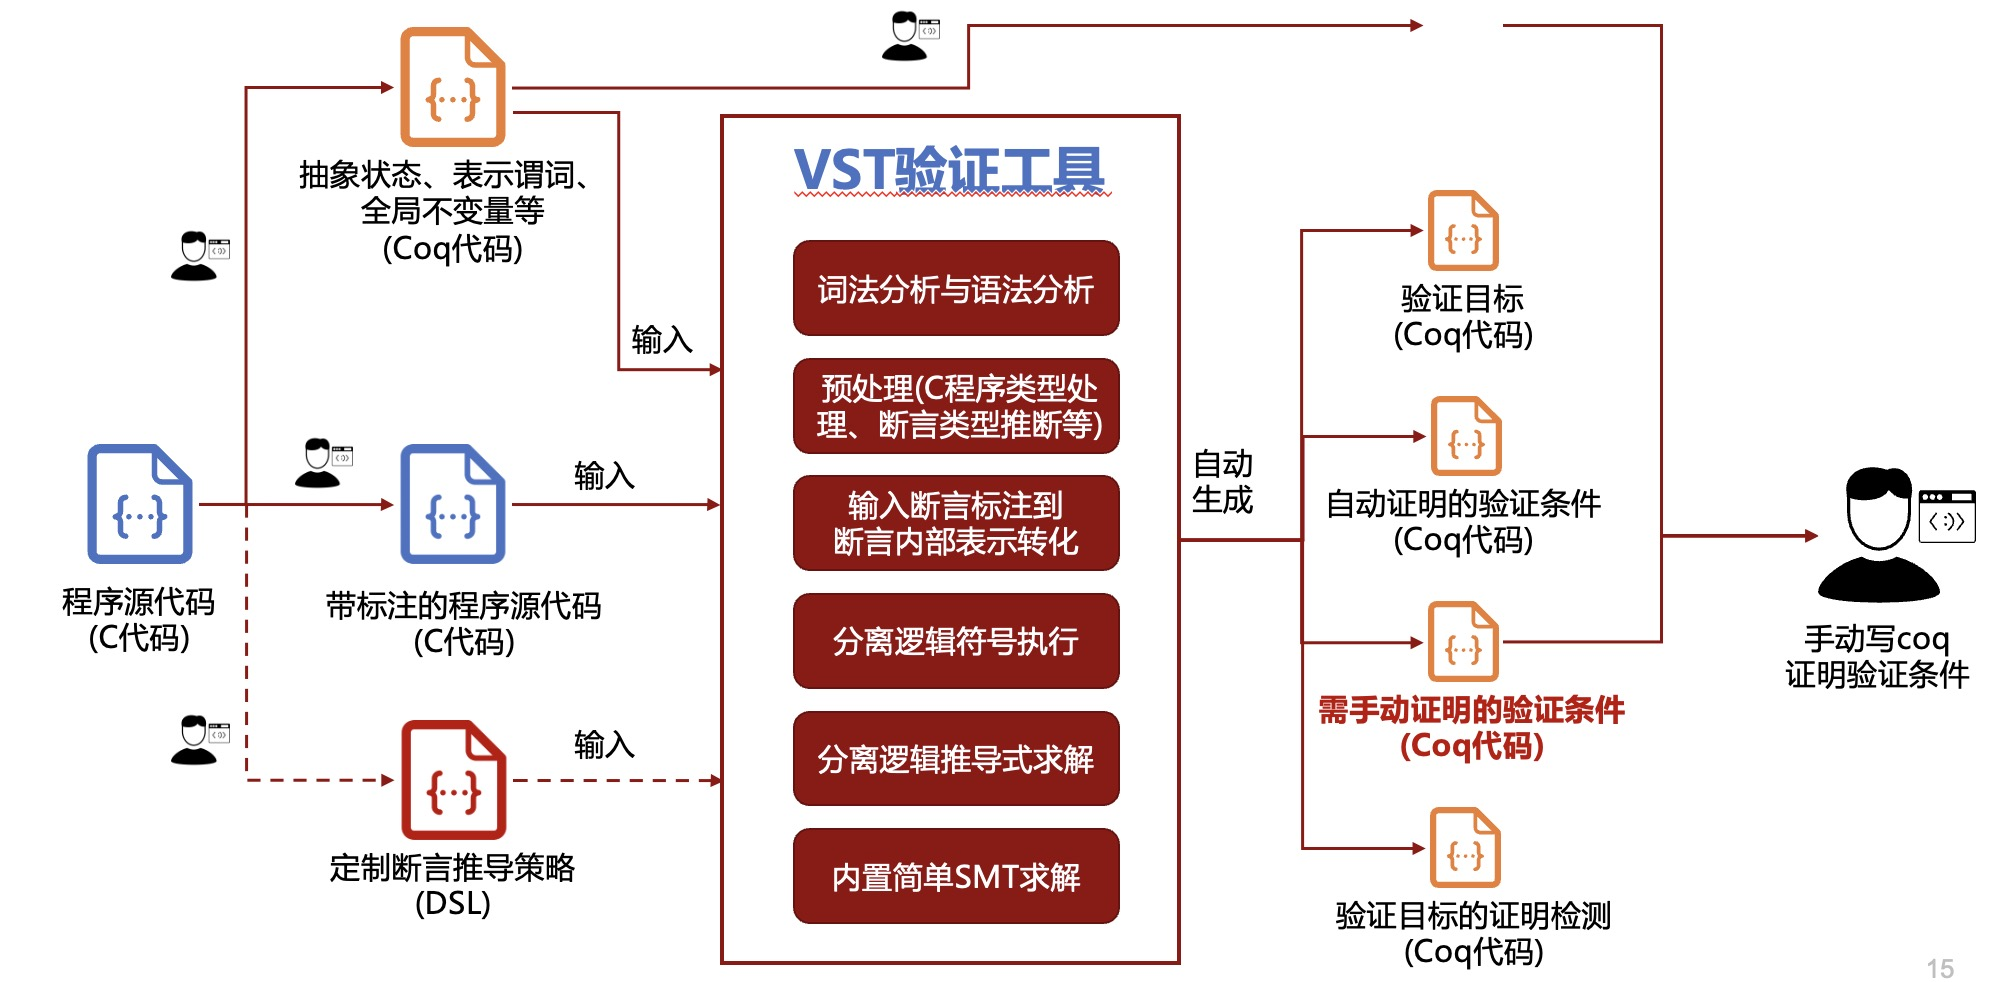
\includegraphics[width=0.9\textwidth]{./fig/vst-flow.png}
    \caption{验证流程核心阶段示意图}
    \label{fig:vst-flow}
\end{figure}

\begin{itemize}
    \item \textbf{建模规约}
    \begin{itemize}
        \item 在Coq中定义数据结构的内存模型(如链表、缓冲区等);
        \item 建立全局不变量与函数级形式化规约;
        \item 编制strategy,指导VST执行验证策略,简化验证过程;
    \end{itemize}

    \item \textbf{自动化验证}
    \begin{itemize}
        \item 通过VST执行符号生成验证条件;
        \item 应用内置SMT求解器处理基础约束;
    \end{itemize}

    \item \textbf{人工介入}
    \begin{itemize}
        \item 处理VST执行符号执行后无法自动证明的验证;
        \item 编写Coq证明脚本,完成复杂验证条件的证明;
    \end{itemize}
\end{itemize}

\subsection{分离逻辑与VST应用}
\label{subsec:sep-vst}

本研究采用VST验证工具实施程序验证,具体流程包含以下三个阶段,各阶段需研究者完成的核心任务如下:

\subsection{建模规约阶段}
\label{subsec:preparation}
本阶段在Coq中建立程序的形式化模型,具体实施包含以下核心内容:
\begin{enumerate}
    \item \textbf{数据结构建模}
    \begin{itemize}
        \item 在Coq中定义C数据结构:
        \begin{figure}[h]  % 位置参数:h此处,t顶部,b底部,p独立页
            \centering  % 居中图片
            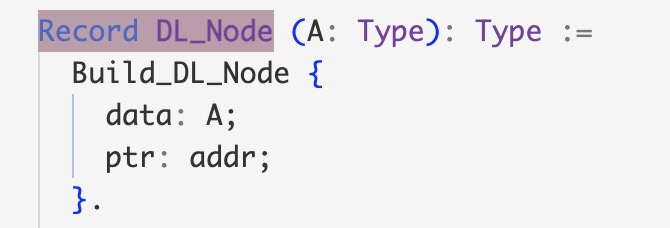
\includegraphics[width=0.8\textwidth]{./fig/Record_dll.png}  % 调整宽度为文本宽度的80%
            \caption{双向链表定义}  % 图片标题
            \label{fig:Record_dll}  % 用于交叉引用的标签
        \end{figure}
        \item 在Coq中定义全局不变量:
        \begin{figure}[h]  % 位置参数:h此处,t顶部,b底部,p独立页
            \centering  % 居中图片
            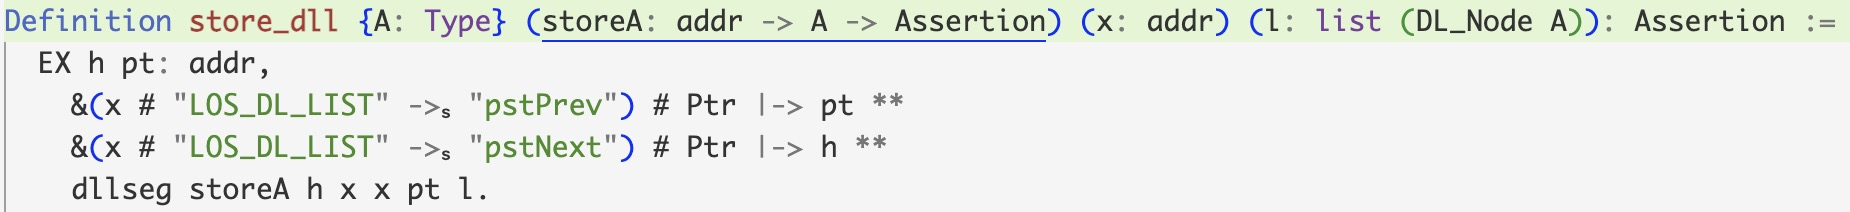
\includegraphics[width=0.8\textwidth]{./fig/store_dll.png}  % 调整宽度为文本宽度的80%
            \caption{store\_dl函数定义与断言示意图}  % 图片标题
            \label{fig:store-dl}  % 用于交叉引用的标签
        \end{figure}
        \item 在C源代码中插入形式化标注:
        \begin{figure}[h]  % 位置参数:h此处,t顶部,b底部,p独立页
            \centering  % 居中图片
            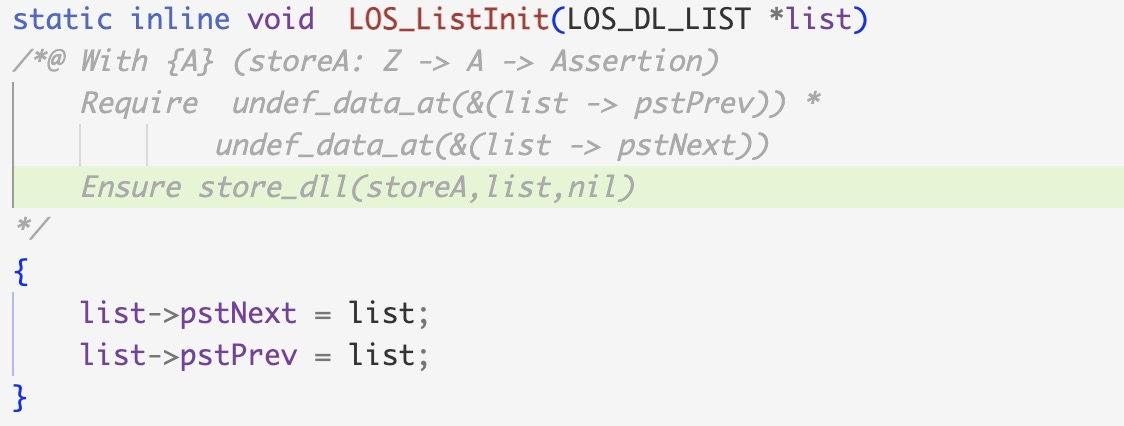
\includegraphics[width=0.8\textwidth]{./fig/LOS_ListInit.png}  % 调整宽度为文本宽度的80%
            \caption{函数形式化标注}  % 图片标题
            \label{fig:LOS_ListInit}  % 用于交叉引用的标签
        \end{figure}
        \item 编写VST验证推导策略:
        \begin{figure}[H]  % 位置参数:h此处,t顶部,b底部,p独立页
            \centering  % 居中图片
            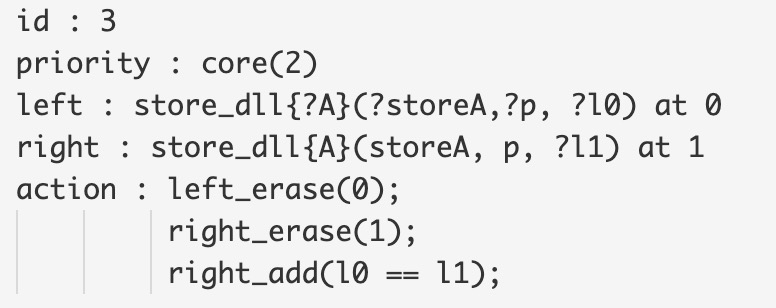
\includegraphics[width=0.8\textwidth]{./fig/store_dll_strategy.png}  % 调整宽度为文本宽度的80%
            \caption{VST Strategy}  % 图片标题
            \label{fig:store_dll_strategy}  % 用于交叉引用的标签
        \end{figure}
    \end{itemize}
\end{enumerate}

\subsection{验证执行阶段}
\label{subsec:execution}

本阶段通过VST工具实现程序验证,具体流程如下:

\begin{enumerate}
    \item \textbf{验证文件生成}
    \begin{itemize}
        \item 输入标注的C代码与验证策略后,生成四类核心文件:
        \begin{itemize}
            \item \texttt{xxx\_proof\_goal}:所有待证明结论列表
            \item \texttt{xxx\_proof\_auto}:已经通过strategy和SMT solver自动解决的相关证明
            \item \texttt{xxx\_proof\_manual}:需要手动完成的相关证明
            \item \texttt{xxx\_proof\_check}:所有证明都已经完成的检查文件汇总
        \end{itemize}
    \end{itemize}

    \item \textbf{自动验证处理}
    \begin{itemize}
        \item 内置符号执行引擎遍历程序路径
        \item 应用验证策略处理基础验证(如内存地址有效性验证)
    \end{itemize}

    \item \textbf{人工验证实施}
    \begin{itemize}
        \item 使用Coq对较复杂的SMT无法自动完成验证的条件进行验证。
        \item 将多个函数的证明合并在一起之后使用Coq进行统一验证,以确保整个系统各个函数调用时系统的正确性。
    \end{itemize}
\end{enumerate}

\section{操作系统建模与形式化规约}
\subsection{内存管理模块的形式化验证}

\noindent VST-IDE通过分离逻辑对动态内存管理进行形式化规约与验证,具体流程如下:

\subsubsection{堆分配器规约}
\begin{equation}
\hoare{\mathrm{emp}}{\mathtt{malloc}(n)}{\exists p.\ \mathrm{valid\_ptr}(p) \ast \mathrm{block}(p, n)}
\end{equation}
\noindent 其中:
\begin{itemize}
    \item $\mathrm{emp}$ 表示空堆断言
    \item $\mathrm{valid\_ptr}(p)$ 保证指针$p$的有效性
    \item $\mathrm{block}(p, n)$ 声明$p$指向大小为$n$字节的连续内存块
    \item $\ast$ 为分离逻辑合取运算符
\end{itemize}

\subsubsection{自动化验证实现}
生成Coq验证代码:
\begin{itemize}
    \item \texttt{*\_proof\_goal.v}(VST-IDE生成的验证目标)
    \item \texttt{*\_proof\_auto.v}(VST-IDE自动证明的命题)
    \item \texttt{*\_proof\_manual.v}(用户使用Coq交互式证明器需要证明的命题)
\end{itemize}

\subsection{进程隔离机制的验证方法}
\label{subsec:proc-isolation}

\subsubsection{能力模型(Capability Model)}
\label{subsubsec:capability-model}

\noindent 定义进程资源归属谓词:
\begin{equation}
\mathrm{ProcRes}(p) \triangleq \ast_{r \in \mathrm{Res}(p)} \mathrm{own}(r,\,p)
\end{equation}
\noindent 其中:
\begin{itemize}
    \item $\mathrm{Res}(p)$ 表示进程$p$拥有的资源集合
    \item $\mathrm{own}(r,\,p)$ 声明资源$r$归属进程$p$,满足:
        \begin{equation}
        \mathrm{own}(r,\,p) \triangleq r \hookrightarrow_p \mathrm{meta}(p)
        \end{equation}
    \item $\ast$ 为分离逻辑的迭代合取运算符,满足:
        \begin{equation}
        \ast_{i=1}^n P_i \equiv P_1 \ast \cdots \ast P_n
        \end{equation}
\end{itemize}

\subsubsection{隔离性定理}
\begin{equation}
\forall p_1 \neq p_2,\ \mathrm{ProcRes}(p_1) \ast \mathrm{ProcRes}(p_2) \vdash \bot
\end{equation}
\noindent 该定理保证:
\begin{itemize}
    \item 分离性:$\mathrm{Res}(p_1) \cap \mathrm{Res}(p_2) = \emptyset$,进程间资源互斥
    \item 无干扰性:进程无法访问不归属于自己的资源
\end{itemize}
\subsection{循环不变式描述}
\section*{程序状态形式化描述}

首先,循环不变式有两条必须满足的性质,即可达性和归纳性。此外,在程序验证中,我们一般还要求循环不变式可证明需要验证的属性。接下来,我们将使用以下的例子,结合形式化的定义,来介绍以上这些性质。

\begin{lstlisting}[language=C++, caption=示例程序]
// to ten
int i = 0;
while(i < 10) { // Inv(i): 0 <= i <= 10
    i = i + 1;
}
assert(i == 10);
\end{lstlisting}

为了形式化地定义循环不变式,我们先做以下定义:

\begin{itemize}
    \item 用 $X$ 来表示程序变量的值,$X$ 可以被理解成一个由程序中所有变量组成的元组(Tuple),或者向量(Vector)
    
    \item 用 $Pre(X)$ 表示循环前的代码对程序变量值的约束
    
    \item 用 $Inv(X)$ 表示循环不变式对程序变量值的约束
    
    \item 用 $G(X)$(Guard)表示循环条件对程序变量值的约束
    
    \item 用 $T(X, X')$ 表示循环体代码对程序变量值的修改,其中 $X'$ 表示被循环体修改后的程序变量的值
    
    \item 用 $Post(X)$ 表示循环后的代码对程序变量值的约束,一般为所需要验证的属性对程序变量值的要求
\end{itemize}
\subsection*{可达性}
可达性实质上是要求,循环不变式表示的状态集合,即$\mathit{Inv}(X)$应该包含所有经过循环前的代码所能到达的状态所形成的集合,即状态集合$\mathit{Pre}(X)$。

\begin{equation}
\forall X.\; \mathit{Pre}(X) \Rightarrow \mathit{Inv}(X)
\end{equation}

\paragraph{示例}
在这个例子中,循环头前的代码形成的约束为$i = 0$。这就意味着,不变式应该包含所有满足$i = 0$的状态。事实上,$0 \leq i \leq 10$包含$i = 0$,即:
$$
\{0\} \subset \{0, 1, \ldots, 10\}
$$
因此可达性成立。

\begin{equation}
\forall i.\; (i = 0) \Rightarrow (0 \leq i \leq 10)
\end{equation}

\subsection*{归纳性}
归纳性是循环不变式最重要的性质,它要求任何被包含在循环不变式中的状态,经过循环后,得到的新状态仍然落在循环不变式中。这个性质保证了循环不变式在任意次循环执行后始终成立。

\begin{equation}
\forall X,X'.\; \left( \mathit{Inv}(X) \land G(X) \land T(X,X') \right) \Rightarrow \mathit{Inv}(X')
\end{equation}

\paragraph{示例验证}
在示例程序中,循环不变式 $0 \leq i \leq 10$ 对应的状态集合为 $\{0,1,\ldots,10\}$。取其中满足循环条件 $i<10$ 的状态 $i=1$,经过循环体后得到 $i'=2$,仍然满足:

$$
\{2\} \subseteq \{0,1,\ldots,10\}
$$

使用逻辑公式验证该不变式的归纳性:
\begin{align*}
\forall i.\; &(0 \leq i \leq 10 \land i < 10) \\
&\Rightarrow 0 \leq i+1 \leq 10
\end{align*}

\paragraph{重要结论}
满足归纳性的不变式可能有多个,但需选择能验证程序属性的:
\begin{itemize}
    \item \textbf{有效不变式}:$0 \leq i \leq 10$ 和 $i \leq 10$ 均可证明 \texttt{assert(i==10)}
    \item \textbf{无效不变式}:$i \leq 20$ 满足可达性和归纳性,但无法证明最终状态 $i=10$
\end{itemize}

\subsection*{可证明性}
该性质要求当循环不变式中的状态满足循环终止条件时,必须满足待验证的程序属性。形式化定义为:

\begin{equation}
\forall X.\; \mathit{Inv}(X) \land \neg G(X) \Rightarrow \mathit{Post}(X)
\end{equation}

\paragraph{示例验证}
在示例程序中,应用具体参数得到验证式:
\begin{align*}
\forall i.\; &(0 \leq i \leq 10) \land \neg(i < 10) \\
&\Rightarrow (i = 10)
\end{align*}

\paragraph{逻辑等价转换} 该式可简化为:
$$
\forall i.\; (0 \leq i \leq 10) \land (i \geq 10) \Rightarrow (i = 10)
$$
在整数域上,该蕴含式等价于:
$$
\{10\} \subseteq \{10\}
$$
因此公式有效。

\subsection{操作规约}
\section{基于VST验证流程}
\subsection{操作系统资源建模}
\subsection{函数条件与断言}
\subsection{验证过程与结果分析}
\section{主要验证内容}
\subsection{基本数据结构-链表}
\subsection{基于链表的操作系统核心模块}
\section{本章小结}
% vim:ts=4:sw=4
    \chapter{动态内存模块验证}
\section{内存模块设计与实现}
\subsection{内存分配与释放}
\subsection{核心机制}

\section{形式化规约}
\subsection{资源分离描述}
\subsection{操作规约}

\section{基于VST的验证过程}
\subsection{内存验证的具体步骤}
\subsection{证明步骤与难点分析}

\section{验证结果}
\subsection{正确性证明}

    %% 正文中的附录部分
    \appendix
    % 要使参考文献列表参与章节编号,可将“bibintoc”改为“bibnumbered”
    \printbibliography[heading=bibintoc]
    \chapter{附录示例}


    %% 以下为正文之后的部分,默认不进行章节编号
    \backmatter
    \ifnoblind
        \chapter{攻读硕士学位期间参与的科研项目}
\noindent [1] 时序因果性医学知识图谱构建和复杂关系获取,科技创新2030-“新一代人工智能”重大项目,项目编号2020AAA0109402\\
\noident [2] 通过形式化全验证的OphenHarmony Liteos-M,项目编号1.3.3

        % Copyright (c) 2014,2016 Casper Ti. Vector
% Public domain.

\chapter{致谢}
首先,我要感谢北京大学给予我学习的机会与场所。在北大的三年时光中,遇见了很多人,经历过很多事,认识到世界的宽广。这段时间谈不上一帆风顺,有迷茫,也有挫折,但也正是这迷茫与挫折,给予我重新审视自己、审视环境的契机。\\
\indent 非常感谢赵海燕老师和张伟老师。
赵老师给予我在软工所窥探科研奥秘的机会,总能认真地聆听我不成熟的想法,并提供实用的意见与建议。
张老师和赵老师在科研、写作、汇报、生活等方面给予我诸多指导,在日常科研工作中为我们指明方向。
张老师对表达的要求、对逻辑的把控、对治学的严谨、对科研的追求,令我受益匪浅。
赵老师对北大自由精神的传承和体现,让我收获颇丰。非常感谢焦文品老师在论文写作中提供的帮助和支持。\\
\indent 感谢潘熙师兄,在学习、工作、生活中给予我无私的帮助与鼓励,在学一前的漫谈和在家三的前后端联调,终将成为美好的回忆。
感谢周衍师兄和渠吉超师兄,引领我踏入众多不曾涉足的领域,深刻体会到世界之大无奇不有,新燕园活动室里多个举杯共饮的下午,必是此生宝贵的财富。
感谢许多的同学,与你们的相识令最后两年校园生活愈发丰富多彩,走遍北小营村探求美食的光景,始终让人忍俊不禁。\\
\indent 感谢张明悦师兄、褚文杰师姐、罗懿行师姐、刘坤师兄、樊梦丹师姐、俞蔼伦同学、刘伟同学、施亦凡同学、陈显彩同学、曲思睿同学以及黄博弈同学等课题组同学们在学习、工作等方面的诸多帮助。\\
\indent 感谢1726实验室里一届又一届的同学们,与你们相处的五年时光是一段愉快的经历。感谢八年时光中在28楼和42楼相遇的九位舍友,感谢你们在生活中对我的包容与帮助。感谢516寝室的四位同学,与你们的缘分是我本科求学路上珍贵的收获。\\
\indent 最后感谢我的父母,感谢父母尊重我的每一个选择,给予我无条件的支持与鼓励。远在他乡求学多年,未能给予你们足够的陪伴,对此深表歉意。在此向你们献上最诚挚的感谢。\\
\indent 有缘再会。

% vim:ts=4:sw=4

        {
    \ctexset{section = {
        format+ = {\centering}, beforeskip = {40bp}, afterskip = {15bp}
    }}
    \specialchap{北京大学学位论文原创性声明和使用授权说明}

    % 学校书面要求本页面不要页码,但在给出的 Word 模版中又有页码。
    % 此处以学校书面要求为准。
    \thispagestyle{empty}
    \mbox{}\vspace*{-3em}
    \section*{原创性声明}

    本人郑重声明:
    所呈交的学位论文,是本人在导师的指导下,独立进行研究工作所取得的成果。
    除文中已经注明引用的内容外,
    本论文不含任何其他个人或集体已经发表或撰写过的作品或成果。
    对本文的研究做出重要贡献的个人和集体,均已在文中以明确方式标明。
    本声明的法律结果由本人承担。
    \vskip 1em
    \rightline{%
        论文作者签名:\hspace{5em}%
        日期:\hspace{2em}年\hspace{2em}月\hspace{2em}日%
    }

    \section*{%
        学位论文使用授权说明\\[-0.33em]
        \textmd{\zihao{5}(必须装订在提交学校图书馆的印刷本)}%
    }

    本人完全了解北京大学关于收集、保存、使用学位论文的规定,即:
    \begin{itemize}
        \item 按照学校要求提交学位论文的印刷本和电子版本;
        \item 学校有权保存学位论文的印刷本和电子版,
            并提供目录检索与阅览服务,在校园网上提供服务;
        \item 学校可以采用影印、缩印、数字化或其它复制手段保存论文;
        \item 因某种特殊原因须要延迟发布学位论文电子版,
            授权学校 $\Box$\nobreakspace{}一年 /
            $\Box$\nobreakspace{}两年 /
            $\Box$\nobreakspace{}三年以后,在校园网上全文发布。
    \end{itemize}
    \centerline{(保密论文在解密后遵守此规定)}
    \vskip 1em
    \rightline{%
        论文作者签名:\hspace{5em}导师签名:\hspace{5em}%
        日期:\hspace{2em}年\hspace{2em}月\hspace{2em}日%
    }

    % 若须排版二维码,请将二维码图片重命名为“barcode”,
    % 转为合适的图片格式,放在 fig 目录下,然后去掉下面 2 行的注释。
    % \vfill\noindent
    % \includegraphics[height = 5em]{fig/barcode}
}

    \fi

\end{document}
